\chapter{Proposta de trabalho}

O levantamento bibliogr�fico mostrou que a �rea de acessibilidade em
sistemas \textit{web} ainda apresenta grandes desafios. Entre eles, podemos
citar:

\begin{itemize}
  \item entregar produtos acess�veis que cubram 100\% das
  defici�ncias e dificuldades;
  \item testar a acessibilidade dos \textit{sites};
  \item implementar plenamente as diretrizes de acessibilidade nos produtos;
  \item mensurar o qu�o acess�vel um \textit{site} �;
  \item escolher a melhor m�trica de avalia��o de acessibilidade;
  \item definir arquiteturas de produtos e servi�os j� existentes de forma que
  agreguem acessibilidade;
  \item conscientizar o desenvolvedor da import�ncia da acessibilidade nos
  produtos;
  \item fornecer ambientes que de fato auxiliem desenvolvedores a entregar
  produtos acess�veis.
\end{itemize}

Podemos observar que os desafios citados anteriormente se relacionam com o
usu�rio final ou com o desenvolvedor. Neste trabalho, optou-se por escolher
a abordagem do desenvolvedor, confeccionando uma ferramenta (\textit{plugin})
para o ambiente de desenvolvimento integrado \textit{Eclipse}.

O trabalho foi motivado pela pesquisa realizada por
\cite{Trewin:2010:ACT:1805986.1806029}, indicando a insatisfa��o dos
desenvolvedores com as ferramentas dispon�veis de desenvolvimento, considerando
a integra��o de acessibilidade ao produto.
Os autores j� possuem experi�ncia com uma ferramenta de avalia��o de \textit{sites} \citep{branco:09}, bem como a
utiliza��o de m�tricas de acessibilidades na avalia��o \citep{branco:11}. Essa
experi�ncia ser� �til para o desenvolvimento do trabalho.

\section{Cronograma}

As atividades abaixo relacionadas ser�o executadas como parte da
metodologia para que os objetivos sejam alcan�ados:

\begin{enumerate}
  \item complementar a pesquisa bibliogr�fica;
  \item escrever e apresentar a qualifica��o;
  \item identificar os pontos de integra��o entre as atividades de Engenharia de
  Requisitos e gera��o de c�digo;
  \item estudar a confec��o de \textit{plugins} para o \textit{Eclipse};
  \item criar e integrar o \textit{plugin} com o \textit{Eclipse};
  \item efetuar testes preliminares da ferramenta;
  \item comparar com outras ferramentas existentes;
  \item efetuar estudos de caso utilizando a ferramenta desenvolvida;
  \item analisar os resultados;
  \item elaborar e publicar artigos cient�ficos;
  \item escrever e defender a disserta��o.
\end{enumerate}

O cronograma das atividades que j� foram
realizadas neste trabalho e as atividades previstas � apresentado a seguir,
considerando as tarefas elencadas anteriormente.

\begin{figure}[htbp]
\centering
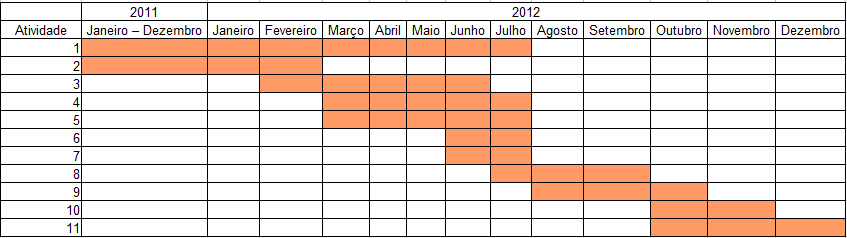
\includegraphics[width=1.0\textwidth]{./images/cronograma.png}
\caption{Cronograma das atividades}
\label{fig:cronograma}
\end{figure}